% !TEX root = ../main.tex

\section{Method}
\label{sec:orga8a42f5}

\mdr{In this section we introduce the Sigmoid F1 Loss. We proceed as follows.}
\daan{We need some example numbers and/or some figures to explain our approach here.}

For a class of multilayer perceptron \(\mathcal{F}(\cdot ; \Theta): \mathcal{X} \rightarrow \mathcal{Y}\), we consider a special case, where \(\mathbf{x} = \{x_1, ..., x_n\}\). Each observation is attributed one or more classes out of a label set \(\mathbf{l} = \{l_1, ..., l_c\}\). Labels \(y_{i}^{j}\) are available for each observation \(i\) and class \(j\). 

For each observation \(i\), label class probabilities can be defined based on predictions as

\todo{check this formula}

\begin{equation}
\mathbf{p}_{i}=\left\{\begin{array}{ll}\hat{\mathbf{y}} & \text { if } y=1 \\ 1-\hat{\mathbf{y}} & \text { otherwise }\end{array}\right.
\end{equation}

Let \(tp\) and \(fp\) be number of true and false positives respectively. It is necessary to define a bound \(b\), at which a prediction is dichotomized:

\todo{note that tn have no effect}

\begin{equation}
\label{eq:conf}
 t p=\sum_{i \in Y^{+}} \mathds{1}_{\mathbf{p_i} \geq b} \quad f p=\sum_{i \in Y^{-}} \mathds{1}_{\mathbf{p_i} \geq b} \quad fn = \sum_{i \in Y^{+}} \mathds{1}_{\mathbf{p_i} < b}
\end{equation}

\(\mathds{1}_{\mathbf{p_i} \geq b}\), \(\mathds{1}_{\mathbf{p_i} < b}\) are thus the count of positive and negative predictions at threshold \(b\), 

We also define precision and recall

\begin{equation}
\begin{aligned} P &=\frac{t p}{t p+f p} \\ R &=\frac{t p}{t p+f n}=\frac{t p}{\left|Y^{+}\right|} \end{aligned}
\end{equation}

We can then define \(F_\beta\), which can be expressed as the effectiveness of retrieval with respect to a user who attaches \(\beta\) times as much importance to recall than precision \cite{informationRetrieval}.

\doubt{maybe ignore $F_\beta$ and only mention $F_1$}

\begin{equation}
F_{\beta}=\left(1+\beta^{2}\right) \frac{P \cdot R}{\beta^{2} P+R}
\end{equation}

Or equivalently:

\begin{equation}
\begin{aligned} F_{\beta} &=\left(1+\beta^{2}\right) \frac{t p}{\left(1+\beta^{2}\right) t p+\beta^{2} f n+f p} \\ &=\left(1+\beta^{2}\right) \frac{t p}{\beta^{2}|Y+|+t p+f p} \end{aligned}
\end{equation}

Given the presence of the step indicator function \(\sum \mathds{1}_{\mathbf{p_i} \geq b}\), \(F_\beta\) is not differentiable for gradient based methods. One way of surpassing that problem is to use a smooth surrogate.

\subsection{soft F1 score}
\label{sec:org3ca83ef}

It is possible define a \emph{soft F1} score \cite{softF1} \doubt{can we cite a Medium post?} with smooth confusion matrix entries (i.e. \(tp\), \(fp\) and \(fn\) are not natural numbers anymore):

$$
\overline{tp}=\sum \hat{\mathbf{y}} \odot \mathbf{y} \quad \overline{fp} = \sum \hat{\mathbf{y}} \odot (\mathbf{1}- \mathbf{y}) \quad \overline{fn} = \sum (\mathbf{1} - \hat{\mathbf{y}}) \odot \mathbf{y}
$$

\begin{equation}
\mathcal{L}_{\text {softF1}}= \frac{\overline{tp}}{2 \overline{tp}+ \overline{fn}+ \overline{fp}}
\end{equation}

\(tp\), \(fp\) and \(fn\) are now replaced by rough surrogates, this method has the advantage of 

% /softF1/ is
% $$\mathcal{L}_{\text {Pred}}=\sum_{i, j}\left(\mathbf{y}_{i j}-\hat{\mathbf{y}}_{i j}\right)^{2}$$

\subsection{sigmoidF1 score}
\label{sec:orgc5d29d7}


\begin{figure}[htbp]
\centering
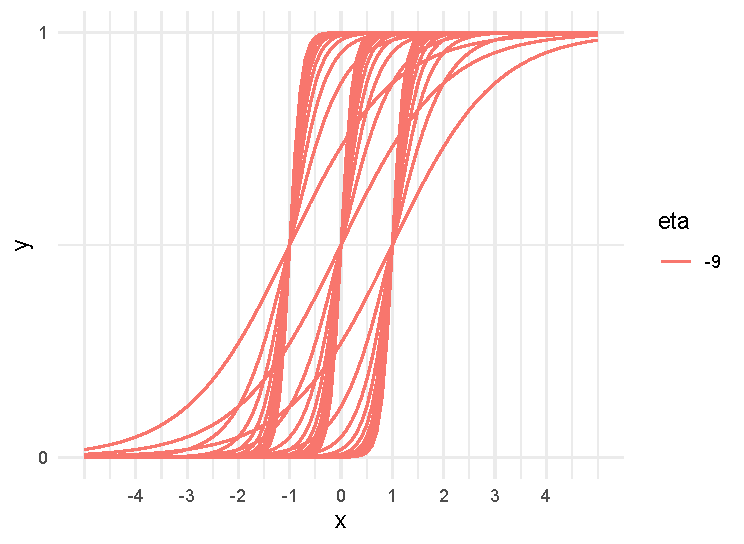
\includegraphics[width=.9\linewidth]{./images/sigmoid.pdf}
\caption{\label{fig:sigmoid}
Sigmoid function with different values for $\beta$ (steepness) \& $\eta$ (offset)}
\end{figure}

We define \emph{sigmoidF1}, inspired by the \emph{Maximum F1-score criterion} for automatic mispronunciation detection \cite{sigmoid}. Whereas a sigmoid function \(S(u)\)

\begin{equation}
S(u; \beta, \eta)=\frac{1}{1+\exp (-\beta (u + \eta))},
\end{equation}

with \(\beta\) and \(\eta\) tunable parameters for slope and offset respectively. Higher \(\beta\) results in steeper slope at the center of the sigmoid and thus more stringent thresholding. At its extreme, \(lim_{\beta\to\infty} S(u; \beta, \eta)\) corresponds to the step function used in Equation \ref{eq:conf}. with \(S(u)\), the confusion matrix entries then become

\begin{equation}\label{eq:sigmoidF1}
\widetilde{tp}=\sum S(\hat{\mathbf{y}}) \odot \mathbf{y} \quad\widetilde{fp}= \sum S(\hat{\mathbf{y}}) \odot (\mathbf{1} - \mathbf{y}) \quad \widetilde{f n}= \sum (\mathbf{1} - S(\hat{\mathbf{y}})) \odot \mathbf{y}
\end{equation}

And thus

\begin{equation}
\mathcal{L}_{\text {sigmoidF1}}= \frac{\widetilde{tp}}{2 \widetilde{tp}+ \widetilde{fn}+ \widetilde{fp}}
\end{equation}

\doubt{mention smooth hinge loss} \cite{smoothHinge}

For \emph{sigmoidF1} \(\beta\) and \(\eta\) are tuned globally as hyperparameters. \emph{SAdF1} (Sigmoid Adaptive F1), is an alternative where \(\beta\) is first set to a relatively low value and increased after each epoch. This way, a loose threshold first allows Stochastic Gradient Descent (SGD) to broadly scan the parameter space accross several local minima, before narrowing parameter search down to a promissing region (similarily to adaptive learning rates).

\emph{SBayesF1} (sigmoid Bayes F1) replaces point estimates for \(\beta\) and \(\eta\) with posterior distribution estimates. 

\begin{equation}
\dot{S}(u_i) = \frac{1}{1+\exp (-\beta_i (u_i + \eta_i))}
\end{equation}

$$ \beta_i \sim N(0, \sigma^{2}_{\beta}) $$

$$ \eta_i \sim N(0, \sigma^{2}_{\eta}) $$

\(\beta_i\) and \(\eta_i\) are estimated with MCMC at training time of the neural network. They are therefore implicitely allowed to vary across examples. The \(\dot{tp}\), \(\dot{fp}\) and \(\dot{fn}\) surrogates can be formulated similarly to Equation \ref{eq:sigmoidF1}. We thus have

\begin{equation}
\mathcal{L}_{\text {SBayesF1}}= \frac{\dot{tp}}{2 \dot{tp}+ \dot{fn}+ \dot{fp}}
\end{equation}


% $\doublewidetilde{tp}$
% https://tex.stackexchange.com/questions/321231/double-widetilde
% doesn't work

\todo{try SadF1 and SBayesF1 in practice}


\subsection{Robustness}
\label{sec:org6c7c3d0}


Similarly to the focal loss \cite{focalLoss}, sigmoidF1 loss deals with class imbalance, robustness to outliers.

\todo{statistical robustness assessment}



\subsection{Evaluation Metrics}
\label{sec:org23c8447}

\mdr{Should this be here or in the Exp Setup section?}

The metrics described below are a result of a survey of different common practices for measuring accuracy of multilabel prediction. When true positives and false positives are used, recall that \(t p=\sum_{i \in Y^{+}} \mathds{1}_{\mathbf{p_i} \geq b}\) and \(f p=\sum_{i \in Y^{-}} \mathds{1}_{\mathbf{p_i} \geq b}\), and thus a threshold \(b\) must be set. When \(b = 0.5\), as is commonly done \todo{add source}, a risk remains that a lot of examples remain without predictions.

Extending \(F_1\) to multi-class binary classification amounts to deciding wether to un/pool classes.
In a first pooled iteration, micro \(F_1\) [SOURCE HERE] equates to creating a single 2x2 confusion matrix for all classes:
$$F_1^{micro} = \frac{\sum tp_c}{2 \sum tp_c + \sum fn_c + \sum fp_c} \quad for \quad c \in C$$

Macro \(F_1\) \cite{threshForF1} amounts to creating one confusion matrix per class or unpooling:

$$F_1^{macro} = \frac{1}{c} \sum_{j=1}^c F_1$$

\doubt{Do we need to justify optimizing for an F1 surrogate at training time and to then use F1 itself as a metric?}
% $$F_1^{macro} = \frac{\sum tp_c}{2 \sum tp_c + \sum fn_c + \sum fp_c} \quad for \quad c \in C$$

Weighted macro \(F_1\) \todo{find source} is similar but includes weighing to account for class imbalance, i.e. weighing each class by the number of groundtruth positives.
\begin{equation}
F_1^{weighted} = \frac{1}{c} \sum_{j=1}^c n_j F_1 \text{ where } n_j = \sum_i \mathds{1}_{\mathbf{y_i^j} = 1}.
\end{equation}

% $$F_1^{weighted} = \frac{\sum tp_c}{2 \sum tp_c + \sum fn_c + \sum fp_c} \quad for \quad c \in C$$

Accuracy is the overall fraction of correctly predicted labels \cite{threshForF1}:

$$
A c c=\frac{t p+t n}{t p+t n+f p+f n}
$$

Note that accuracy assigns equal cost to false positives and false negatives. This is particularly problematic in an unbalanced setup like here.

% - 'samples':
% Calculate metrics for each instance, and find their average (only meaningful for multilabel classification where this differs from accuracy_score).

% $$F_1^{micro} = \frac{\sum tp_c}{2 \sum tp_c + \sum fn_c + \sum fp_c} \quad for \quad c \in C$$

More variations scores exist in the literature, such as hamming loss~\cite{hammingLoss} (the fraction of incorrectly predicted labels), hamming score.q


\todo{compare to this:} \cite{lossComp}

\todo{Hamming Loss}
\todo{Precision@K, Recall@K, NDCG@K}
\todo{MLTSVM loss and the three-way loss inspired by it} \cite{MLTSVM} and \cite{MLTSVMThreeway}

\todo{explain batch size mathematically for F1 surrogate losses}
%%% Local Variables:
%%% mode: latex
%%% TeX-master: "../main"
%%% End:
